\section{Rete per uno Stabilimento Balneare}%
\label{sec:rete}

Ci viene chiesto di progettare una rete LAN per uno stabilimento balneare. Ho progettato la rete con Cisco Packet Tracer utilizzando la versione 8.0-2, la topologia della rete \`e inclusa in questo documento nella sotto-sezione~\ref{sub:topologia}.

Ho scelto di dividere la rete dello Stabilimento Balneare in due sottoreti. La prima, che ho chiamato \emph{LAN Amministrazione}, contiene la rete utilizzata dai dipendenti con completo accesso a Internet. All'interno di questa rete ho incluso anche il server DHCP che si occupa della gestione dell'intera rete.

La seconda sottorete l'ho dedicata alla rete Wireless. Ho ipotizzato che lo stabilimento balneare in questione offrisse l'accesso Wi-Fi gratuito per buona parte della spiaggia oltre che nel ristorante infatti ho anche previsto l'installazione di \emph{Access Point} per l'esterno in parte dello Stabilimento.







\begin{landscape}
    \subsection{Topologia}%
    \label{sub:topologia}
    \thispagestyle{empty}
    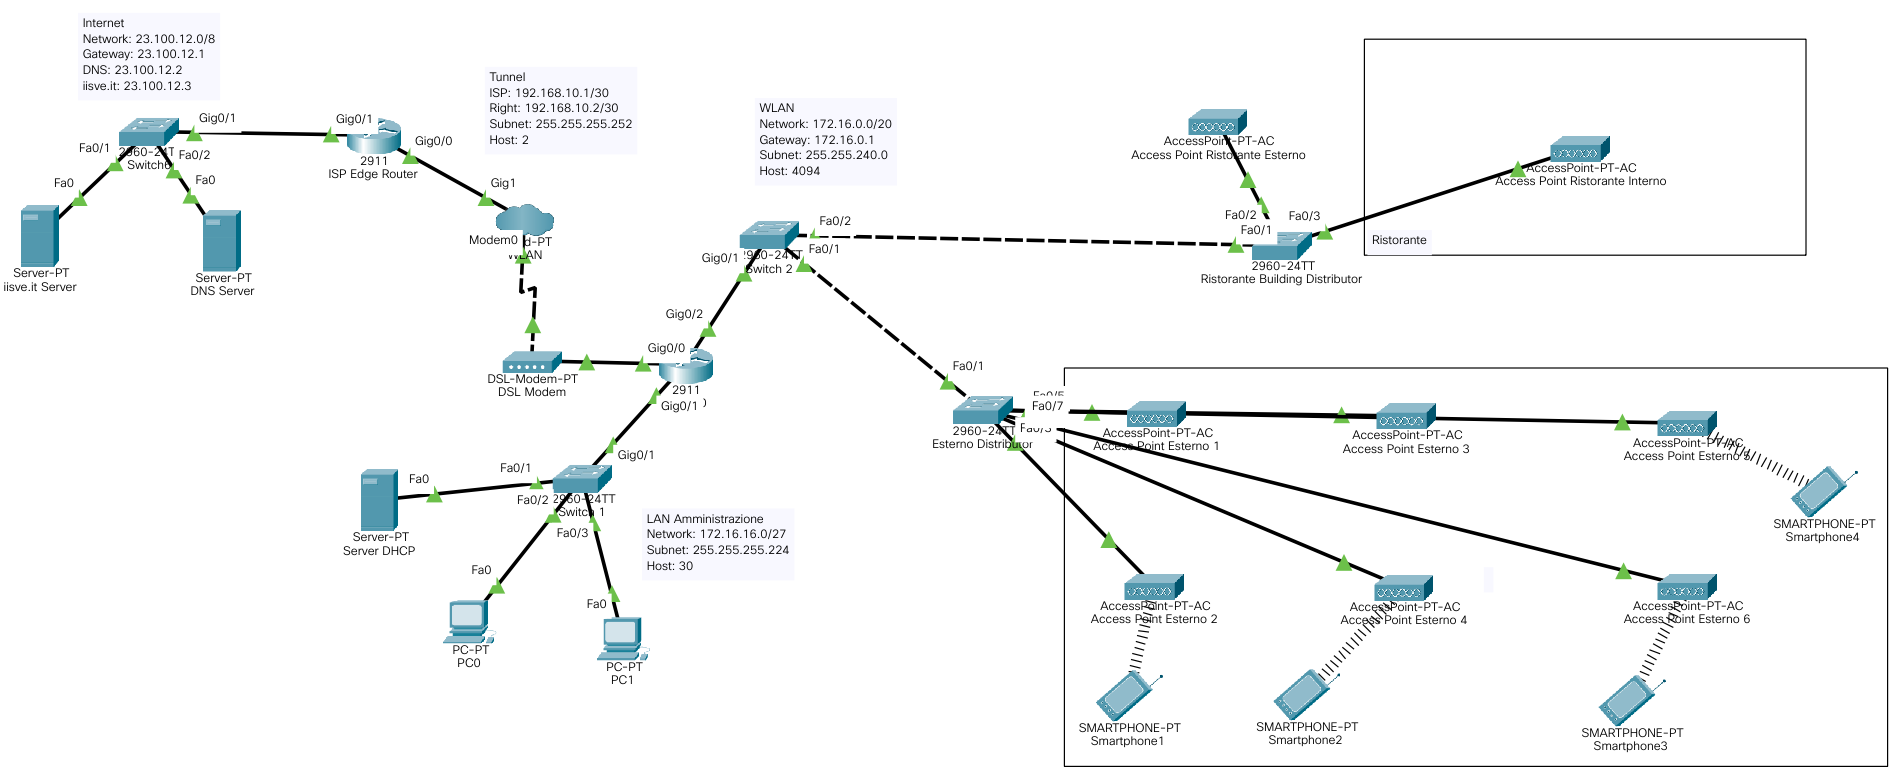
\includegraphics[width=\linewidth]{rete.png}
\end{landscape}